\documentclass[12pt, a4paper]{article}
\usepackage{enumitem}
\setlist[enumerate]{label = (\roman*)}
\usepackage{amsmath}
\usepackage{mathtools}
\usepackage{amssymb}
\usepackage{amsthm}
\theoremstyle{definition}
\newtheorem{example}{Example}

\usepackage{tikz}
\usepackage{hyperref}

\newcommand{\summation}[2]{\sum\limits_{#1}^{#2}}
\newcommand{\limit}[2]{\lim\limits_{#1\to #2}}
\newcommand{\vep}{\varepsilon}
\newcommand{\union}[2]{\cup_{#1}^{#2}}
\newcommand{\m}[1]{\mathcal{#1}}
\newcommand{\minus}{\textbackslash}
\newcommand{\intersection}[2]{\cup_{#1}^{#2}}

\begin{document}
\begin{example}[Funny property]
If $\union{i=1}{\infty}A_i=M$(universal set), then each $A_i\in\mathcal{A}$.
\begin{proof}
Say $B_1,\dots\notin\m{A}$, whereas $C_1,\dots\in\m{A}$,  then $\union{i=1}{\infty}B_i=M\minus (\union{i=1}{\infty}C_i)\in\m{A}$. Contradiction yields.
\end{proof}
\end{example}

\begin{example}[Non-uniquness of $\sigma$-algebra]
Notice that for a given set $M$, the $\sigma$-algebra on $M$ is not unique. $\m{P}(M)$ and $\{M,\emptyset\}$ are $\sigma$-algebras  on $M$.
\end{example}

\begin{example}[Half-interval in $2$-dimensional space]
This example aims to demonstrate half-interval in a $2$-dimensional space. Consider 
\[
]0,1]:\{x\in\mathbb{R}^2:0<x\leq 1\}.
\]
\begin{figure}[h!]
\centering
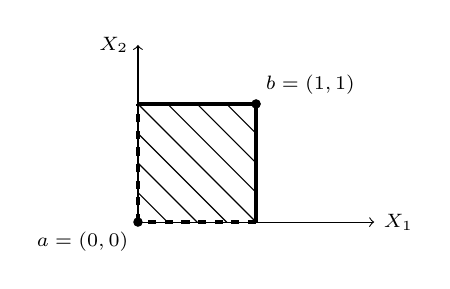
\begin{tikzpicture}[scale = 1.5, font = \scriptsize]
\draw [<->] (0,1.5) node [left] {$X_2$} -- (0,0) -- (2,0) node [right] {$X_1$};
\node [below left] at (0,0) {$a=(0,0)$};
\node [above right] at (1,1) {$b=(1,1)$};
\draw [fill] (0,0) circle (1pt);
\draw [fill] (1,1) circle (1pt);
\draw [ultra thick, dashed] (0,0) -- (0,1);
\draw [ultra thick, dashed] (1,0) -- (0,0);
\draw [ultra thick] (0,1) -- (1,1);
\draw [ultra thick] (1,1) -- (1,0);
\clip (0,0) rectangle (1,1);
\foreach \x in {-1,-0.75,-0.5,-0.25,0,0,0.25,0.5,0.75,1,1.25,1.5,1.75,2,2.25,2.5,2.75}
\draw [xshift = \x cm] (-2, 2) -- (2,-2);
\end{tikzpicture}
\caption{$2$-dimension half interval}
\end{figure}
\end{example}

\begin{example}
Besides $]a,b]$, there are also other intervals considered to be Borel set.
\begin{enumerate}
\item 
$\mathbb{R}$ is a Borel set.
\begin{proof}
It's clear that $]-\infty,n]$ for $n=1,2,\dots$ is Borel set. Then, from the fact that $\m{B}$ is a $\sigma$-algebra on $\mathbb{R}$, we can conclude:
\[
\mathbb{R}=\union{n=1}{\infty}\,]-\infty,n]\in\m{B}.
\]
\end{proof}
\item $\{a\}$ for all $a\in \mathbb{R}$ is a Borel set.
\begin{proof}
Let $A_n = ]a-\frac{1}{n},a]\in\m{B}$, then $\intersection{n=1}{\infty}A_n = \{a\}\in\m{B}$.
\end{proof}
\item $[a,b]$ for all $-\infty<a<b<\infty$ is a Borel set.
\begin{proof}
$(a,b],\{a\}$ are Borel sets, therefore $[a,b] = (a,b]\cup\{a\}$ is a Borel set.
\end{proof}
\end{enumerate}
\end{example}

\begin{example}[A $\pi$-system needs not to be a $\sigma$-algebra.]
Let $M=\{1,2\}$. Clearly, $\Big\{ \emptyset,\{1\}\Big\}$ is a $\pi$-system, but it fails to be a $\sigma$-algebra.
\end{example}

\begin{example}[$\max\{U,V\}$ can be a simple function]
If $U,V\in\m{S}_+$, then $\max\{U,V\}$ and $\min\{U,V\}\in\m{S}_+$.
\begin{proof}
Intuitively thinking, $\max\{U,V\}$ should admit finite value and is a nonnegative function as well. 

Now we give a formal proof. First, assume $U(x) = \summation{i=1}{n}\alpha_i1_{A_i}$, $V(x) = \summation{j=1}{m}\beta_i1_{B_i}$, where $A_i$  are disjoint and $\union{i=1}{n}A_i=M$, same for $B_j$. 
Notice that: 
\begin{align*}
U(x)&=\summation{i=1}{n}\alpha_i1_{A_i}\\
&=\summation{i=1}{n}\alpha_i1_{\union{j=1}{m}(A_i\cap B_j)}\\
&=\summation{i=1}{n}\alpha_i\summation{j=1}{m}1_{A_i\cap B_j}\\
&=\sum_{i,j}\alpha_i1_{A_i\cap B_j}.
\end{align*}
Same argument, 
\[
V(x) = \sum_{i,j}\beta_j1_{A_i\cap B_j}
\]
Therefore,
\[
\max\{f,g\}=\sum_{i,j}\max\{\alpha_i,\beta_j\}1_{A_i\cap B_j}\in\m{S}_+.
\]

\end{proof}
\end{example}



























\end{document}